\documentclass[aspectratio=169, 11pt]{beamer}

% --- Theme ---
\usetheme{metropolis}
\usepackage{appendixnumberbeamer}
\usepackage{amsmath,amssymb,bm}
\usepackage{booktabs}
\usepackage{tikz}
\usetikzlibrary{arrows.meta, positioning, calc, decorations.pathreplacing,
                 overlay-beamer-styles}
\usepackage{graphicx}

% --- Colors ---
\definecolor{accent}{RGB}{0, 100, 170}
\definecolor{highlight}{RGB}{200, 60, 30}
\definecolor{darkgreen}{RGB}{0, 120, 60}
\setbeamercolor{alerted text}{fg=highlight}

% --- Fonts ---
\setbeamerfont{title}{size=\Large, series=\bfseries}
\setbeamerfont{frametitle}{size=\large}

% --- Commands ---
\newcommand{\eps}{\varepsilon}
\newcommand{\mean}[1]{\langle #1 \rangle}
\newcommand{\highlight}[1]{\textcolor{highlight}{\textbf{#1}}}
\newcommand{\good}[1]{\textcolor{darkgreen}{#1}}
\newcommand{\bad}[1]{\textcolor{highlight}{#1}}

% --- Title ---
\title{Closed-Form Mean-Element Theory for GEqOE}
\subtitle{The Direct Residue Decomposition Method}
\author{Jose Manuel Montilla Garc\'ia}
\date{2026}
\institute{}

\begin{document}

% =====================================================================
\maketitle

% =====================================================================
\begin{frame}{The Problem}

Propagating satellite orbits under gravitational perturbations is
\textbf{expensive}:

\begin{itemize}\setlength{\itemsep}{0.1em}
    \item Osculating integration resolves every orbital revolution
    \item For a LEO satellite: $\sim$16 orbits/day, $\sim$5{,}800/year
    \item For catalog maintenance: $\sim$25{,}000 objects $\times$ 7 days
          $= 2.8 \times 10^6$ orbit-revolutions
\end{itemize}

\vspace{0.2em}
\textbf{Goal}: replace osculating integration with an
\alert{analytical theory} that:

\begin{enumerate}\setlength{\itemsep}{0.1em}
    \item Propagates smooth, slowly varying \emph{mean} elements
          (huge step sizes)
    \item Reconstructs the full osculating state at any desired epoch
          via closed-form corrections
\end{enumerate}

\vspace{0.2em}
\textbf{Classical approach}: Brouwer (1959) --- canonical variables,
Lie transforms, closed-form $J_2$--$J_5$.\\[0.1em]
\textbf{This work}: same goal, different elements (GEqOE), different
method (\alert{direct residue decomposition}).

\end{frame}

% =====================================================================
\section{Setup: GEqOE and the Averaging Idea}

% =====================================================================
\begin{frame}{Generalized Equinoctial Orbital Elements (GEqOE)}

\textbf{State vector} (Ba\`u et al.\ 2021):
\[
\bm y = (\nu,\; p_1,\; p_2,\; K,\; q_1,\; q_2)
\]

\begin{columns}[T]
\column{0.52\textwidth}
\begin{itemize}
    \item $\nu$ --- generalized mean motion (energy)
    \item $p_1, p_2$ --- eccentricity vector
    \item $K$ --- generalized eccentric longitude (\alert{fast angle})
    \item $q_1, q_2$ --- inclination vector
\end{itemize}

\column{0.45\textwidth}
\textbf{Key properties}:
\begin{itemize}
    \item[\good{$\checkmark$}] No singularity at $e = 0$
    \item[\good{$\checkmark$}] No singularity at $i = 0$
    \item[\good{$\checkmark$}] No critical-inclination singularity
    \item[\good{$\checkmark$}] Fast angle $K$ is explicit
    \item[\bad{$\times$}] Singular at $i = 180^\circ$ (retrograde equat.)
\end{itemize}
\end{columns}

\vspace{0.5em}
Under the unperturbed Kepler problem: $\dot K = w/r$ (fast),
everything else constant.

\end{frame}

% =====================================================================
\begin{frame}{Orbit Geometry from $K$}

All geometric quantities are \textbf{explicit functions of $K$}:

\begin{align*}
r &= a\bigl(1 - p_1 \sin K - p_2 \cos K\bigr)
& &\text{radius} \\[4pt]
X &= a\bigl(\alpha p_1 p_2 \sin K + (1-\alpha p_1^2)\cos K - p_2\bigr)
& &\text{in-plane } x \\[4pt]
Y &= a\bigl(\alpha p_1 p_2 \cos K + (1-\alpha p_2^2)\sin K - p_1\bigr)
& &\text{in-plane } y
\end{align*}

where $g = \sqrt{p_1^2 + p_2^2}$, \;
$\beta = \sqrt{1 - g^2}$, \;
$\alpha = 1/(1+\beta)$.

\vspace{0.5em}
\textbf{Crucial observation}:
$r$, $X$, $Y$ are all \alert{affine in $\sin K$ and $\cos K$}.

\vspace{0.3em}
This means the zonal forcing (which depends on powers of $r$,
$X$, $Y$, and $\hat z = f(X, Y, q_1, q_2)/r$) is a
\textbf{trigonometric-rational function of $K$}.

\end{frame}

% =====================================================================
\begin{frame}{The Averaging Idea}

\textbf{Separate fast from slow}:
\vspace{-0.5em}
\[
\underbrace{K}_{\text{fast, once per orbit}}
\qquad
\underbrace{\nu, p_1, p_2, q_1, q_2}_{\text{slow, secular/long-period}}
\]

\vspace{-0.4em}
The \textbf{orbital average} over one revolution in $K$:
\vspace{-0.3em}
\[
\mean{f}_K
= \frac{1}{2\pi a}\int_0^{2\pi} r(K)\,f(K)\,dK
= \frac{1}{2\pi}\int_0^{2\pi} f(M)\,dM
\]

\vspace{-0.4em}
\textbf{First-order averaged system} (mean elements $\bar{\bm z}$):
\vspace{-0.3em}
\[
\dot{\bar{\bm z}} = \eps\,\bar{\bm f}_1(\bar{\bm z})
\qquad \longleftarrow \quad
\text{smooth, slowly varying, large time steps}
\]

\vspace{-0.4em}
But the averaged theory needs \textbf{two more ingredients}:
\begin{enumerate}\setlength{\itemsep}{0.1em}
    \item A map: \; osculating $\to$ mean \; (initialization)
    \item A map: \; mean $\to$ osculating \; (reconstruction)
\end{enumerate}

\vspace{-0.3em}
These are the \alert{short-period corrections} --- and computing them
analytically is the hard part.

\end{frame}

% =====================================================================
\section{The Near-Identity Transformation}

% =====================================================================
\begin{frame}{Mean $\leftrightarrow$ Osculating: The Short-Period Map}

Write the near-identity transformation:
\begin{align*}
\bm z_{\text{osc}} &= \bar{\bm z}
+ \eps\,\bm u_1(\bar{\bm z}, \bar K) + O(\eps^2)
& &\text{(forward map)} \\[4pt]
\bar{\bm z} &= \bm z_{\text{osc}}
- \eps\,\bm u_1(\bm z_{\text{osc}}, K_{\text{osc}}) + O(\eps^2)
& &\text{(inverse map)}
\end{align*}

\vspace{-0.3em}
The correction $\bm u_1$ satisfies the \textbf{homological equation}:
\[
\boxed{
\frac{\partial \bm u_1}{\partial \bar K}
= \frac{\bar r}{\bar w}
\Bigl[
\bm f_1(\bar{\bm z}, \bar K)
- \bar{\bm f}_1(\bar{\bm z})
\Bigr]
}
\]

\vspace{0.2em}
\textbf{Translation}: $\bm u_1$ is the antiderivative (in $K$) of the
\emph{oscillatory part} of the forcing, weighted by $r/w = dt/dK$.

\vspace{0.3em}
The forcing $\bm f_1$ is a rational-trigonometric function of $K$.\\
The weight $r/w$ is also a trigonometric function of $K$.\\[0.2em]
$\Rightarrow$ We need to \alert{integrate rational-trigonometric functions
of $K$} in closed form.

\end{frame}

% =====================================================================
\begin{frame}{The Integration Challenge}

The short-period integrals look like:
\[
\bm u_1(\bar K)
= \int^{\bar K}
\frac{r(\phi)}{w}
\left[
\bm f_1(\bar{\bm z}, \phi)
- \bar{\bm f}_1(\bar{\bm z})
\right] d\phi
\]

\vspace{-0.3em}
For a zonal potential of degree $n$:
\begin{itemize}\setlength{\itemsep}{0.1em}
    \item $\bm f_1$ involves $P_n(\hat z)$ ---
          a polynomial of degree $n$ in $\sin u$
    \item Times $1/r^{n+1}$ --- a power of $(1 - g\cos G)$
    \item Times $r/w$ --- the Jacobian weight
\end{itemize}

\vspace{0.3em}
The classical approach: \textbf{tangent-half-angle substitution}
$t = \tan(G/2)$.\\
$\Rightarrow$ Rational integrals in $t$, solvable in principle.\\
$\Rightarrow$ But the expressions \alert{explode in complexity} for $n \ge 3$.

\vspace{0.5em}
\begin{center}
\large
\textit{Is there a better integration variable?}
\end{center}

\end{frame}

% =====================================================================
\section{The Key Insight: Complex True Anomaly}

% =====================================================================
\begin{frame}{Enter the Complex True Anomaly}

Define $F = e^{if}$ where $f$ is the true anomaly.

\vspace{0.3em}
\textbf{The M\"obius map} connects $F$ to $z = e^{iG}$
(eccentric anomaly exponential):
\[
F = \frac{z - q}{1 - qz},
\qquad
z = \frac{F + q}{1 + qF},
\qquad
q = \frac{g}{1+\beta}
\]

\vspace{-0.3em}
On the physical orbit, both $z$ and $F$ trace the \alert{unit circle}
$|F| = 1$ as $K$ advances by $2\pi$.

\vspace{0.5em}
\textbf{Three structural advantages of $F$}:

\begin{enumerate}\setlength{\itemsep}{0.3em}
    \item The zonal forcing is a \good{Laurent polynomial} in $F$
          (not a rational-trigonometric function requiring substitutions)

    \item The Jacobian $dM/dF$ has a \good{fixed pole structure}
          (independent of the zonal degree $n$)

    \item The short-period integral becomes a \good{contour integral}
          of a rational function
\end{enumerate}

\end{frame}

% =====================================================================
\begin{frame}{Why $F$ Makes the Forcing Simple}

\textbf{Zonal forcing} involves powers of $\sin u = \sin(\omega + f)$:
\vspace{-0.2em}
\[
\sin u = \frac{wF - (wF)^{-1}}{2i},
\qquad w = e^{i\omega}
\]

\vspace{-0.4em}
This is a \alert{Laurent monomial} in $F$ (times powers of $w$).

\vspace{0.2em}
$\Rightarrow$ $P_n(\hat z) = P_n(s_i \sin u)$ is a
\textbf{finite Laurent polynomial} in $F$:
\vspace{-0.2em}
\[
P_n(s_i \sin u)
= \sum_{k=-n}^{n} c_k(Q)\, (wF)^k
\]

\vspace{-0.4em}
Combined with $r^{-(n+1)}$ (also rational in $F$), the complete forcing
for each zonal degree $n$ is a \textbf{rational function of $F$}
whose numerator is a Laurent polynomial of bounded degree.

\vspace{0.2em}
\textbf{Comparison}: in $K$, the same forcing involves
nested products of $(1 - g\cos G)^{-k}$ and trigonometric polynomials
--- much harder to manipulate.

\end{frame}

% =====================================================================
\begin{frame}{The Jacobian: Fixed Poles}

The Jacobian between the mean anomaly $M$ and the complex true anomaly
$F$ is:
\[
\boxed{
\frac{dM}{dF}
= -i\,\frac{(1-q^2)^3}{1+q^2}\,
\frac{F}{(F+q)^2(1+qF)^2}
}
\]

\vspace{0.5em}
\textbf{Pole structure}:
\begin{itemize}
    \item Simple zero at $F = 0$
    \item Double pole at $F = -q$ \quad (inside the unit disk, $|{-}q| < 1$)
    \item Double pole at $F = -1/q$ \quad (outside the unit disk)
\end{itemize}

\vspace{0.8em}
\begin{center}
\alert{The denominator $(F+q)^2(1+qF)^2$ is
\textbf{independent of the zonal degree $n$}.}
\end{center}

\vspace{0.5em}
This is the key structural fact: no matter how high the zonal degree,
the integration always has the \textbf{same} pole structure.
Only the numerator grows with $n$.

\end{frame}

% =====================================================================
\section{The Direct Residue Decomposition}

% =====================================================================
\begin{frame}{The Universal Integrand}

For any zonal degree $n$, any slow variable $v$, and any
$\omega$-harmonic $m$, the short-period integral has the form:
\[
u_{1,m}^v(F)
= \int
\underbrace{a_{v,m}(F)}_{\text{Laurent poly in } F}
\cdot
\underbrace{\frac{dM}{dF}}_{\text{fixed poles}}
\; dF
\]

After clearing negative $F$-powers (shift $s = -k_{\min}$):
\[
\boxed{
\text{Integrand} = \text{scale} \times
\frac{N(F)}{F^s\,(F+q)^2\,(1+qF)^2}
}
\]

where $N(F)$ is a polynomial in $F$ with coefficients in $\mathbb{Q}(q, Q)$.

\vspace{0.5em}
\textbf{This is just a rational function!}\\[0.3em]
$\Rightarrow$ Partial fraction decomposition gives the antiderivative
in closed form.

\end{frame}

% =====================================================================
\begin{frame}{The Five-Step Algorithm}

\begin{enumerate}
    \setlength{\itemsep}{0.3em}

    \item \textbf{Polynomial long division}\\
    $N(F) = Q_{\text{poly}}(F) \cdot D(F) + N_{\text{rem}}(F)$,
    \quad $\deg N_{\text{rem}} < \deg D$

    \item \textbf{Double-pole residues} at $F = -q$ and $F = -1/q$\\
    Extract principal parts by evaluation at the poles

    \item \textbf{Residues at $F = 0$} (for shift $s \ge 2$)\\
    Taylor recurrence for the coefficients of
    $N_{\text{rem}}(F)/[(F+q)^2(1+qF)^2]$

    \item \textbf{Assemble antiderivative}\\
    $u_{1,m}^v(F) = \text{polynomial}
    - \dfrac{B}{F+q} - \dfrac{D_c}{q(1+qF)}
    - \sum_{j} \dfrac{E_j}{F^{j-1}} - C$

    \item \textbf{Zero-mean gauge}\\
    Fix the constant $C$ so that $\mean{u_{1,m}^v}_M = 0$
    using structural mean formulas
\end{enumerate}

\vspace{0.3em}
\alert{No logarithmic terms appear} --- guaranteed by the periodicity
of $u_1$ on $|F|=1$ (single-valuedness forces all log coefficients to vanish).

\end{frame}

% =====================================================================
\begin{frame}{Why Logs Cancel: The Geometric Argument}

\begin{columns}[T]
\column{0.55\textwidth}
On the physical orbit, $F$ traces the \textbf{unit circle}
$|F| = 1$ as $M$ advances by $2\pi$.

\vspace{0.3em}
The standard rational integration of $1/(F+q)$ would give $\log(F+q)$.
But $\log$ is multi-valued on a closed contour.

\vspace{0.3em}
\textbf{The guarantee}: $u_1$ must be single-valued (periodic in $M$).
A simple pole at $F = -q$ would produce $\alpha\log(F+q)$, which is
multi-valued on $|F|=1$ (the circle passes on both sides of $-q$).
$\Rightarrow$ $\alpha = 0$.

\vspace{0.3em}
The residue theorem confirms: the contour integral of the
zero-$M$-average integrand times $dM/dF$ has poles only at $F=-q$
and $F=0$ inside the disk. The $F=0$ residue is computable
independently, forcing $\alpha = 0$ and hence $\hat B = 0$.

\vspace{0.3em}
$\Rightarrow$ No logarithms, only \alert{algebraic} antiderivatives.

\column{0.4\textwidth}
\vspace{-0.5em}
\begin{center}
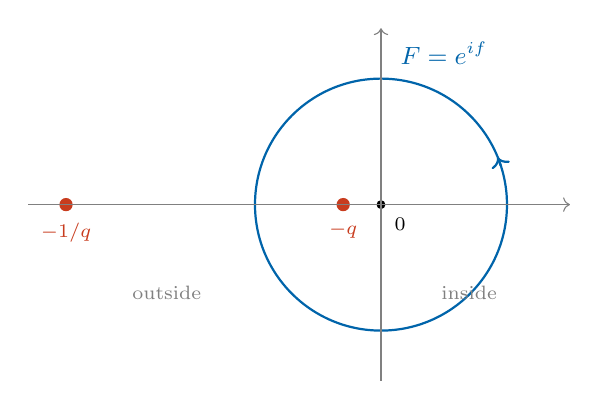
\begin{tikzpicture}[scale=1.6]
    % Unit circle
    \draw[thick, accent] (0,0) circle (1);
    \draw[->, accent, thick] (0.95, 0.31) arc (18:22:1);

    % Poles
    \fill[highlight] (-0.3, 0) circle (1.5pt)
        node[below=3pt, font=\scriptsize] {$-q$};
    \fill[highlight] (-2.5, 0) circle (1.5pt)
        node[below=3pt, font=\scriptsize] {$-1/q$};

    % Origin
    \fill (0,0) circle (1pt)
        node[below right=2pt, font=\scriptsize] {$0$};

    % F arrow
    \node[accent, font=\small] at (0.5, 1.2) {$F = e^{if}$};

    % Labels
    \node[font=\scriptsize, text=gray] at (0.7, -0.7) {inside};
    \node[font=\scriptsize, text=gray] at (-1.7, -0.7) {outside};

    % Axes
    \draw[gray, thin, ->] (-2.8, 0) -- (1.5, 0);
    \draw[gray, thin, ->] (0, -1.4) -- (0, 1.4);
\end{tikzpicture}
\end{center}

\vspace{0.1em}
{\small Periodicity of $u_1$ on the unit circle forces all log
coefficients to vanish identically.}
\end{columns}

\end{frame}

% =====================================================================
\begin{frame}{Why This Scales}

\begin{center}
\begin{tabular}{@{}lrrr@{}}
\toprule
Degree & Forcing terms & Result size & Generation time \\
\midrule
$J_2$ & 14--21 & 18 KB & seconds \\
$J_3$ & 32--36 & 79 KB & $\sim$1 min \\
$J_4$ & 44--55 & 206 KB & $\sim$15 min \\
$J_5$ & 72--78 & 510 KB & $\sim$60 min \\
\bottomrule
\end{tabular}
\end{center}

\vspace{0.2em}
\textbf{The denominator $(F+q)^2(1+qF)^2$ is degree-independent.}

\vspace{0.1em}
As $n$ increases:
\begin{itemize}\setlength{\itemsep}{0.1em}
    \item Only the \emph{numerator} polynomial $N(F)$ grows (linearly in $n$)
    \item Algorithm steps (long division, evaluation, recurrence)
          are polynomial-time in the numerator degree
    \item The \emph{coefficient complexity} in $\mathbb{Q}(q, Q)$ is the
          real cost driver (GCD simplification)
\end{itemize}

\vspace{0.1em}
\textbf{Key optimization}: operations performed
\emph{coefficient-by-coefficient} in the $F$-Laurent expansion.
The 80-min total is a \alert{one-time} cost; results cached and
loaded in $< 5$~s.

\end{frame}

% =====================================================================
\section{The Complete Analytical Theory}

% =====================================================================
\begin{frame}{The Three-Step Pipeline}

\begin{center}
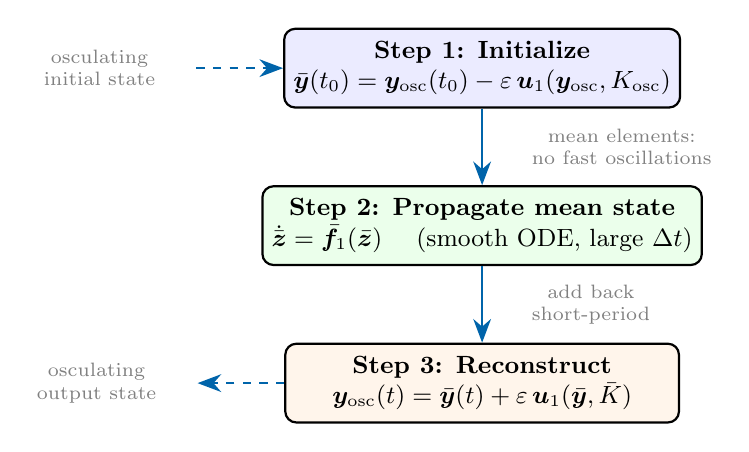
\begin{tikzpicture}[
    box/.style={draw, rounded corners=4pt, minimum width=5cm,
                minimum height=1cm, align=center, font=\small,
                thick},
    arr/.style={-{Stealth[length=3mm]}, thick, accent},
    lbl/.style={font=\scriptsize, text=gray, align=center}
]

\node[box, fill=blue!8] (init) at (0, 0)
    {\textbf{Step 1: Initialize}\\
     $\bar{\bm y}(t_0) = \bm y_{\text{osc}}(t_0)
     - \eps\,\bm u_1(\bm y_{\text{osc}}, K_{\text{osc}})$};

\node[box, fill=green!8] (prop) at (0, -2)
    {\textbf{Step 2: Propagate mean state}\\
     $\dot{\bar{\bm z}} = \bar{\bm f}_1(\bar{\bm z})$
     \quad (smooth ODE, large $\Delta t$)};

\node[box, fill=orange!8] (recon) at (0, -4)
    {\textbf{Step 3: Reconstruct}\\
     $\bm y_{\text{osc}}(t)
     = \bar{\bm y}(t) + \eps\,\bm u_1(\bar{\bm y}, \bar K)$};

\draw[arr] (init) -- (prop)
    node[midway, right=0.5cm, lbl]
    {mean elements:\\no fast oscillations};

\draw[arr] (prop) -- (recon)
    node[midway, right=0.5cm, lbl]
    {add back\\short-period};

\node[lbl, left=1.5cm of init] {osculating\\initial state};
\node[lbl, left=1.5cm of recon] {osculating\\output state};

\draw[arr, dashed] (init.west) ++(-1.1, 0) -- (init.west);
\draw[arr, dashed] (recon.west) -- ++(-1.1, 0);

\end{tikzpicture}
\end{center}

\vspace{0.1em}
Every operation is the evaluation of a \textbf{precomputed algebraic
formula}. No numerical quadrature, no interpolation, no iterative scheme
(except the standard Kepler equation).

\end{frame}

% =====================================================================
\begin{frame}{For Pure $J_2$: Fully Closed-Form}

Under $J_2$ alone, the averaged disturbing function depends only on
$a$, $e$, $i$.\\
$\Rightarrow$ No argument-of-pericenter dependence $\Rightarrow$
\textbf{uniform rotations}:

\vspace{-0.3em}
\[
\begin{bmatrix} \bar p_1(t) \\ \bar p_2(t) \end{bmatrix}
= \begin{bmatrix}
\cos\theta_\Psi & \sin\theta_\Psi \\
-\sin\theta_\Psi & \cos\theta_\Psi
\end{bmatrix}
\begin{bmatrix} \bar p_1(t_0) \\ \bar p_2(t_0) \end{bmatrix},
\qquad
\theta_\Psi = \omega_{\Psi, J_2}(t - t_0)
\]

\vspace{-0.2em}
\begin{itemize}\setlength{\itemsep}{0.1em}
    \item Magnitudes $\bar g$, $\bar Q$ constant
    \item Angles $\bar\Psi$, $\bar\Omega$ advance linearly
    \item No ODE integration needed --- \alert{the mean state is a
          closed-form function of elapsed time}
\end{itemize}

\vspace{0.3em}
For general zonals ($J_3$--$J_5$): the mean system is a smooth
autonomous ODE in $(\bar g, \bar Q, \bar\Psi, \bar\Omega)$, driven by
the single slow angle $\bar\omega = \bar\Psi - \bar\Omega$.\\[0.2em]
Step sizes: \textbf{tens to hundreds of orbital periods}.

\end{frame}

% =====================================================================
\begin{frame}{Validation: Osculating Reconstruction}

\begin{columns}[T]
\column{0.48\textwidth}
\textbf{Low eccentricity} ($e = 0.05$):\\[0.3em]
\begin{itemize}
    \item Position RMS: \good{$\sim$200 m}
    \item Radial error: \good{$\sim$3 m}
    \item 10 orbits, $J_2$--$J_5$
\end{itemize}

\vspace{0.5em}
\textbf{High eccentricity} ($e = 0.65$):\\[0.3em]
\begin{itemize}
    \item Position RMS: $\sim$3 km
    \item Radial error: \good{$\sim$10 m}
    \item 8 orbits, $J_2$--$J_5$
\end{itemize}

\vspace{0.5em}
\textbf{Scaling test}: log-log slope $= 0.998$\\
$\Rightarrow$ errors scale as $O(\eps)$ --- first-order theory confirmed.

\column{0.48\textwidth}
\vspace{-0.5em}
\begin{center}
\includegraphics[width=\textwidth]{../figures/zonal_short_period_scaling.png}
\end{center}
\vspace{-0.5em}
{\scriptsize RMS position error vs.\ zonal scale factor.
Slope $\approx 1$ confirms first-order behavior.}
\end{columns}

\end{frame}

% =====================================================================
\begin{frame}{12-Regime Comparison vs.\ Brouwer--Lyddane}

\begin{center}
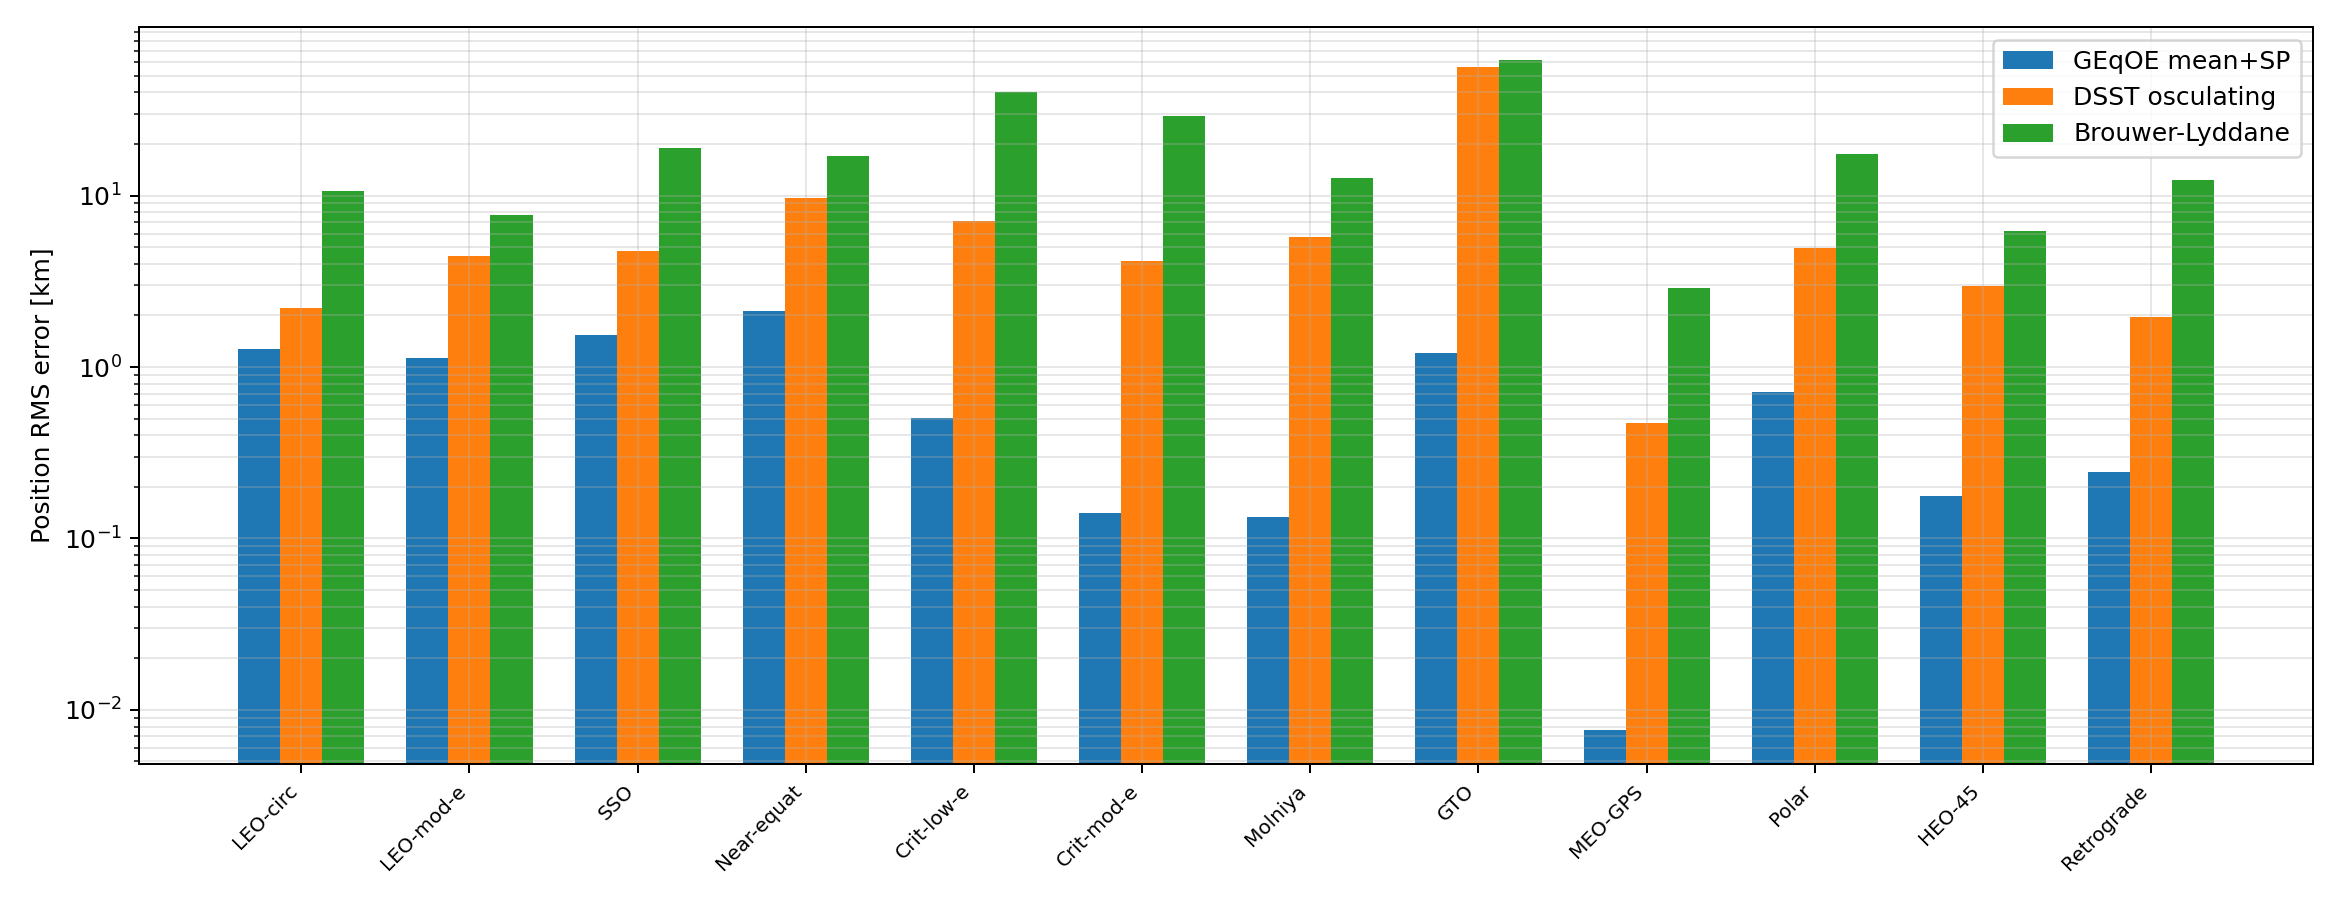
\includegraphics[width=0.78\textwidth]{../figures/extended_validation_comparison_bar.png}
\end{center}

\vspace{-0.3em}
{\small GEqOE theory outperforms Brouwer--Lyddane (Orekit) by
\alert{4$\times$ to 335$\times$} across all 12 regimes.\\
Both compared against Cowell Cartesian truth with identical
$J_2$--$J_5$ constants.}

\end{frame}

% =====================================================================
\section{The Big Picture}

% =====================================================================
\begin{frame}{Why the Residue Decomposition is the Unlocker}

\vspace{-0.3em}
\begin{center}
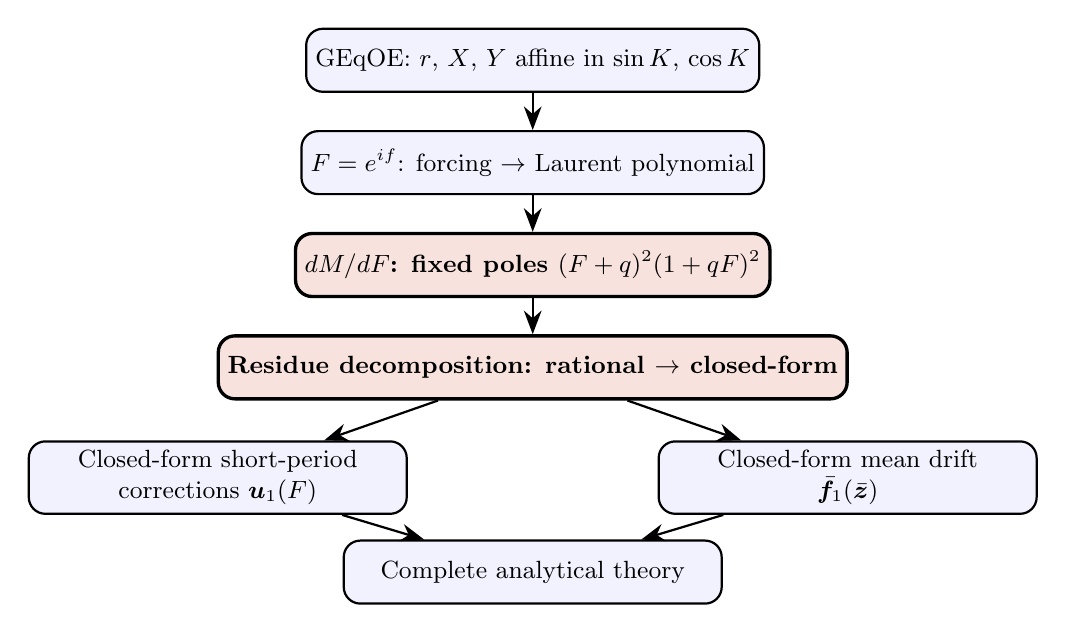
\begin{tikzpicture}[
    concept/.style={draw, rounded corners=6pt, minimum width=4.8cm,
                    minimum height=0.8cm, align=center, font=\small,
                    thick, fill=blue!5},
    key/.style={draw, rounded corners=6pt, minimum width=4.8cm,
                minimum height=0.8cm, align=center, font=\small\bfseries,
                very thick, fill=highlight!15},
    arr/.style={-{Stealth[length=3mm]}, thick},
]

\node[concept] (geqoe) at (0, 3.2)
    {GEqOE: $r$, $X$, $Y$ affine in $\sin K$, $\cos K$};

\node[concept] (fvar) at (0, 1.9)
    {$F = e^{if}$: forcing $\to$ Laurent polynomial};

\node[key] (jacobian) at (0, 0.6)
    {$dM/dF$: fixed poles $(F+q)^2(1+qF)^2$};

\node[key] (residue) at (0, -0.7)
    {\alert{Residue decomposition:}
     rational $\to$ closed-form};

\node[concept] (sp) at (-4, -2.1)
    {Closed-form short-period\\
     corrections $\bm u_1(F)$};
\node[concept] (mean) at (4, -2.1)
    {Closed-form mean drift\\
     $\bar{\bm f}_1(\bar{\bm z})$};
\node[concept] (theory) at (0, -3.3)
    {Complete analytical theory};

\draw[arr] (geqoe) -- (fvar);
\draw[arr] (fvar) -- (jacobian);
\draw[arr] (jacobian) -- (residue);
\draw[arr] (residue) -- (sp);
\draw[arr] (residue) -- (mean);
\draw[arr] (sp) -- (theory);
\draw[arr] (mean) -- (theory);

\end{tikzpicture}
\end{center}

\vspace{0.1em}
Without the residue decomposition $\Rightarrow$ numerical quadrature
(DSST) or truncated series (Hansen).\\
With it $\Rightarrow$ \alert{exact closed-form expressions}, precomputed
once and evaluated at runtime.

\end{frame}

% =====================================================================
\begin{frame}{Extensibility: The Same Method Unlocks Everything}

The pole structure $(F+q)^2(1+qF)^2$ is a property of
\textbf{Keplerian geometry}, not of the perturbation source.

\vspace{0.3em}
$\Rightarrow$ Any perturbation whose forcing is rational in $F$ can be
processed by the same algorithm:

\vspace{0.3em}
\begin{center}
\begin{tabular}{lcc}
\toprule
Perturbation & Rational in $F$? & Mean drift \\
\midrule
Zonal harmonics $J_n$ & \good{Yes} & Autonomous \\
Tesseral harmonics $C_{nm}$, $S_{nm}$
    & \good{Yes} (frozen $\theta_G$) & Non-autonomous \\
Third-body (Sun, Moon)
    & \good{Yes} (frozen $\hat{\bm r}'$) & Non-autonomous \\
Solar radiation pressure
    & \good{Yes} (frozen $\hat{\bm r}_\odot$) & Non-autonomous \\
Fourier-in-$K$ thrust
    & \good{Yes} (by construction) & Controlled \\
\bottomrule
\end{tabular}
\end{center}

\vspace{0.2em}
\textbf{One algorithm, one pole structure, all perturbation sources.}

\end{frame}

% =====================================================================
\begin{frame}{The Road Ahead}

\begin{center}
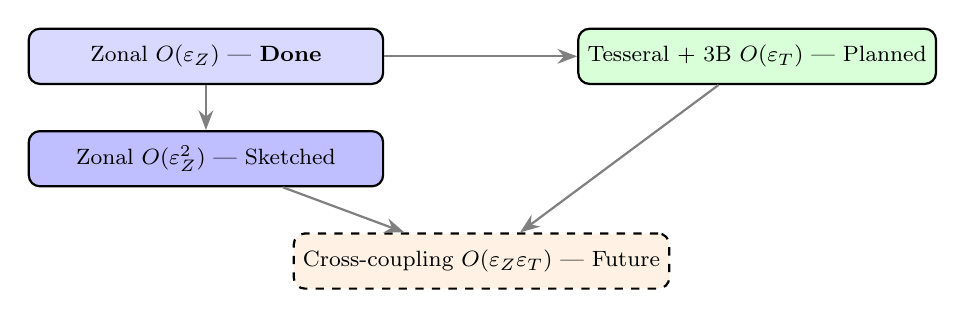
\begin{tikzpicture}[
    box/.style={draw, rounded corners=4pt, minimum width=4.5cm,
                minimum height=0.7cm, align=center, font=\footnotesize,
                thick},
    arr/.style={-{Stealth[length=2.5mm]}, thick, gray},
]

\node[box, fill=blue!15] (z1) at (-3.5, 0)
    {Zonal $O(\eps_Z)$ --- \textbf{Done}};
\node[box, fill=blue!25] (z2) at (-3.5, -1.3)
    {Zonal $O(\eps_Z^2)$ --- Sketched};
\node[box, fill=green!15] (t1) at (3.5, 0)
    {Tesseral + 3B $O(\eps_T)$ --- Planned};
\node[box, fill=orange!10, dashed] (cross) at (0, -2.6)
    {Cross-coupling $O(\eps_Z \eps_T)$ --- Future};

\draw[arr] (z1) -- (z2);
\draw[arr] (z1) -- (t1);
\draw[arr] (z2) -- (cross);
\draw[arr] (t1) -- (cross);

\end{tikzpicture}
\end{center}

\vspace{0.3em}

\begin{itemize}
    \item Each layer is \textbf{independent} --- developed and published
          separately
    \item The residue decomposition is the \textbf{shared engine} across
          all layers
    \item Combined theory:
          $O(\eps_Z^2) + O(\eps_T) + O(\eps_{3B})$ --- captures all
          operationally relevant terms
\end{itemize}

\end{frame}

% =====================================================================
\begin{frame}{Summary}

\begin{enumerate}
    \setlength{\itemsep}{0.4em}

    \item \textbf{GEqOE elements} provide a non-singular fast angle $K$
    with affine orbit geometry

    \item The \textbf{complex true anomaly} $F = e^{if}$ converts the
    forcing to Laurent polynomials

    \item The \textbf{Jacobian $dM/dF$} has a fixed pole structure
    independent of the harmonic degree

    \item The \textbf{direct residue decomposition} converts the
    short-period integrals to exact closed-form rational expressions

    \item The result is a \textbf{fully analytical} mean-element theory:
    precomputed formulas evaluated at runtime, no quadrature

    \item The method \textbf{generalizes} to tesseral harmonics,
    third-body, and thrust --- same poles, same algorithm

    \item Validated: \textbf{4--335$\times$ better} than
    Brouwer--Lyddane across 12 orbital regimes
\end{enumerate}

\end{frame}

% =====================================================================
\appendix
\begin{frame}[standout]
    Thank you
\end{frame}

\end{document}
